\documentclass[french,]{article}
\usepackage{lmodern}
\usepackage{amssymb,amsmath}
\usepackage{ifxetex,ifluatex}
\usepackage{fixltx2e} % provides \textsubscript
\ifnum 0\ifxetex 1\fi\ifluatex 1\fi=0 % if pdftex
  \usepackage[T1]{fontenc}
  \usepackage[utf8]{inputenc}
\else % if luatex or xelatex
  \ifxetex
    \usepackage{mathspec}
  \else
    \usepackage{fontspec}
  \fi
  \defaultfontfeatures{Ligatures=TeX,Scale=MatchLowercase}
\fi
% use upquote if available, for straight quotes in verbatim environments
\IfFileExists{upquote.sty}{\usepackage{upquote}}{}
% use microtype if available
\IfFileExists{microtype.sty}{%
\usepackage{microtype}
\UseMicrotypeSet[protrusion]{basicmath} % disable protrusion for tt fonts
}{}
\usepackage{hyperref}
\hypersetup{unicode=true,
            pdftitle={Rapport TP2 - Design Pattern},
            pdfauthor={Fleury Malik - malik.fleury@he-arc.ch; Wermeille Bastien - bastien.wermeille@he-arc.ch; Bulloni Lucas - lucas.bulloni@he-arc.ch},
            pdfborder={0 0 0},
            breaklinks=true}
\urlstyle{same}  % don't use monospace font for urls
\ifnum 0\ifxetex 1\fi\ifluatex 1\fi=0 % if pdftex
  \usepackage[shorthands=off,main=french]{babel}
\else
  \usepackage{polyglossia}
  \setmainlanguage[]{french}
\fi
\usepackage[top=3cm, bottom=2cm, left=2.5cm, right=3cm]{geometry}
\usepackage{color}
\usepackage{fancyvrb}
\newcommand{\VerbBar}{|}
\newcommand{\VERB}{\Verb[commandchars=\\\{\}]}
\DefineVerbatimEnvironment{Highlighting}{Verbatim}{commandchars=\\\{\}}
% Add ',fontsize=\small' for more characters per line
\newenvironment{Shaded}{}{}
\newcommand{\KeywordTok}[1]{\textcolor[rgb]{0.00,0.44,0.13}{\textbf{{#1}}}}
\newcommand{\DataTypeTok}[1]{\textcolor[rgb]{0.56,0.13,0.00}{{#1}}}
\newcommand{\DecValTok}[1]{\textcolor[rgb]{0.25,0.63,0.44}{{#1}}}
\newcommand{\BaseNTok}[1]{\textcolor[rgb]{0.25,0.63,0.44}{{#1}}}
\newcommand{\FloatTok}[1]{\textcolor[rgb]{0.25,0.63,0.44}{{#1}}}
\newcommand{\ConstantTok}[1]{\textcolor[rgb]{0.53,0.00,0.00}{{#1}}}
\newcommand{\CharTok}[1]{\textcolor[rgb]{0.25,0.44,0.63}{{#1}}}
\newcommand{\SpecialCharTok}[1]{\textcolor[rgb]{0.25,0.44,0.63}{{#1}}}
\newcommand{\StringTok}[1]{\textcolor[rgb]{0.25,0.44,0.63}{{#1}}}
\newcommand{\VerbatimStringTok}[1]{\textcolor[rgb]{0.25,0.44,0.63}{{#1}}}
\newcommand{\SpecialStringTok}[1]{\textcolor[rgb]{0.73,0.40,0.53}{{#1}}}
\newcommand{\ImportTok}[1]{{#1}}
\newcommand{\CommentTok}[1]{\textcolor[rgb]{0.38,0.63,0.69}{\textit{{#1}}}}
\newcommand{\DocumentationTok}[1]{\textcolor[rgb]{0.73,0.13,0.13}{\textit{{#1}}}}
\newcommand{\AnnotationTok}[1]{\textcolor[rgb]{0.38,0.63,0.69}{\textbf{\textit{{#1}}}}}
\newcommand{\CommentVarTok}[1]{\textcolor[rgb]{0.38,0.63,0.69}{\textbf{\textit{{#1}}}}}
\newcommand{\OtherTok}[1]{\textcolor[rgb]{0.00,0.44,0.13}{{#1}}}
\newcommand{\FunctionTok}[1]{\textcolor[rgb]{0.02,0.16,0.49}{{#1}}}
\newcommand{\VariableTok}[1]{\textcolor[rgb]{0.10,0.09,0.49}{{#1}}}
\newcommand{\ControlFlowTok}[1]{\textcolor[rgb]{0.00,0.44,0.13}{\textbf{{#1}}}}
\newcommand{\OperatorTok}[1]{\textcolor[rgb]{0.40,0.40,0.40}{{#1}}}
\newcommand{\BuiltInTok}[1]{{#1}}
\newcommand{\ExtensionTok}[1]{{#1}}
\newcommand{\PreprocessorTok}[1]{\textcolor[rgb]{0.74,0.48,0.00}{{#1}}}
\newcommand{\AttributeTok}[1]{\textcolor[rgb]{0.49,0.56,0.16}{{#1}}}
\newcommand{\RegionMarkerTok}[1]{{#1}}
\newcommand{\InformationTok}[1]{\textcolor[rgb]{0.38,0.63,0.69}{\textbf{\textit{{#1}}}}}
\newcommand{\WarningTok}[1]{\textcolor[rgb]{0.38,0.63,0.69}{\textbf{\textit{{#1}}}}}
\newcommand{\AlertTok}[1]{\textcolor[rgb]{1.00,0.00,0.00}{\textbf{{#1}}}}
\newcommand{\ErrorTok}[1]{\textcolor[rgb]{1.00,0.00,0.00}{\textbf{{#1}}}}
\newcommand{\NormalTok}[1]{{#1}}
\usepackage{graphicx,grffile}
\makeatletter
\def\maxwidth{\ifdim\Gin@nat@width>\linewidth\linewidth\else\Gin@nat@width\fi}
\def\maxheight{\ifdim\Gin@nat@height>\textheight\textheight\else\Gin@nat@height\fi}
\makeatother
% Scale images if necessary, so that they will not overflow the page
% margins by default, and it is still possible to overwrite the defaults
% using explicit options in \includegraphics[width, height, ...]{}
\setkeys{Gin}{width=\maxwidth,height=\maxheight,keepaspectratio}
\IfFileExists{parskip.sty}{%
\usepackage{parskip}
}{% else
\setlength{\parindent}{0pt}
\setlength{\parskip}{6pt plus 2pt minus 1pt}
}
\setlength{\emergencystretch}{3em}  % prevent overfull lines
\providecommand{\tightlist}{%
  \setlength{\itemsep}{0pt}\setlength{\parskip}{0pt}}
\setcounter{secnumdepth}{5}
% Redefines (sub)paragraphs to behave more like sections
\ifx\paragraph\undefined\else
\let\oldparagraph\paragraph
\renewcommand{\paragraph}[1]{\oldparagraph{#1}\mbox{}}
\fi
\ifx\subparagraph\undefined\else
\let\oldsubparagraph\subparagraph
\renewcommand{\subparagraph}[1]{\oldsubparagraph{#1}\mbox{}}
\fi

\title{Rapport TP2 - Design Pattern}
\author{Fleury Malik -
\href{mailto:malik.fleury@he-arc.ch}{\nolinkurl{malik.fleury@he-arc.ch}} \and Wermeille Bastien -
\href{mailto:bastien.wermeille@he-arc.ch}{\nolinkurl{bastien.wermeille@he-arc.ch}} \and Bulloni Lucas -
\href{mailto:lucas.bulloni@he-arc.ch}{\nolinkurl{lucas.bulloni@he-arc.ch}}}
\date{\today}

\begin{document}
\maketitle

{
\setcounter{tocdepth}{5}
\tableofcontents
}
\section{TP2 - Rapport}\label{tp2---rapport}

\subsection{Introduction}\label{introduction}

Pour ce Travail Pratique, il a été demandé de développer un programme de
création de pizza en utilisant les patterns Decorator, Builder et State.

Toutes les classes implémentent l'interface \texttt{Pizza\_I}. Et les 3
patterns sont implémentés dans leur package respectif.

\begin{figure}[htbp]
\centering
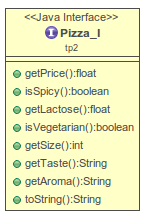
\includegraphics{pizza_i.png}
\caption{Pizza\_I}
\end{figure}

Toutes les classes propres aux patterns ont été préfixées par le nom de
celui-ci afin d'identifier plus facilement quel pattern est utilisé.

\subsection{Decorator}\label{decorator}

Decorator est un pattern qui permet d'ajouter un fonctionnement à un
objet de base.

\subsubsection{Réalisation}\label{ruxe9alisation}

Les decorators représentent les ingrédients et la sauce sur la pizza.
Nous avons donc créé une classe abstraite, \texttt{Decorator} qui
représentent tous les ingrédients et nous avons fait deux classes qui
hérite de \texttt{Decorator}, \texttt{DecoratorSauce} et
\texttt{DecoratorIngredient}. Ces décorateurs sont séparés, car ils ont
un comportement différent. La sauce ne va jamais modifier le prix, car
faisant partie de l'offre de base, contrairement aux ingrédients. Ces
deux classes permettent également de faire de la généralisation et donc
de séparer les sauces des ingrédients rajoutés.

Les décorateurs ont également un énuméré \texttt{Aromas} et
\texttt{Tastes}, qui va permettre de concaténer facilement les
différents types de goût et arômes de chaque ingrédient/sauce.

\paragraph{Ingrédients}\label{ingruxe9dients}

Ensuite nous avons ajouté plusieurs ingrédients qui héritent de
\texttt{DecoratorIngredient}, \texttt{DecoratorBacon},
\texttt{DecoratorHam}, \texttt{DecoratorMozzarella},
\texttt{DecoratorOregano}, \texttt{DecoratorPepper} et
\texttt{DecoratorPepperoni}. Tous ces ingrédients redéfinissent les
fonctions de l'interface \texttt{Pizza\_I} et auront chacun leur propre
prix.

\begin{figure}[htbp]
\centering
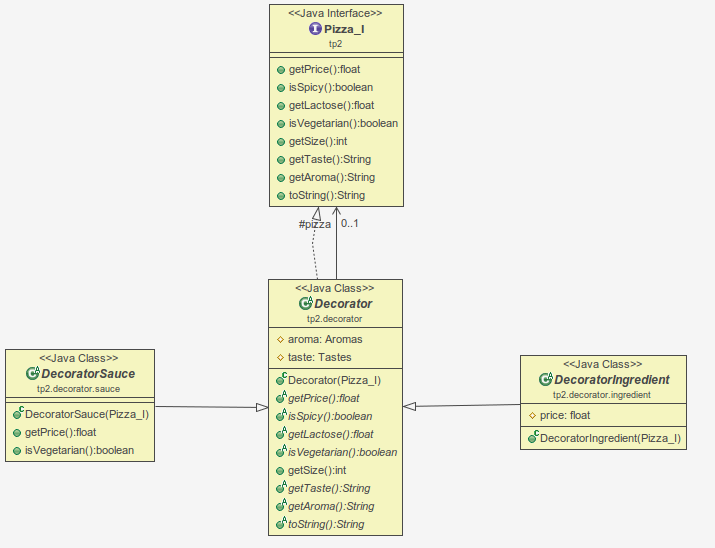
\includegraphics{decoratorglobal.png}
\caption{Decorator}
\end{figure}

\subparagraph{Exemple de code}\label{exemple-de-code}

\begin{Shaded}
\begin{Highlighting}[]
\KeywordTok{public} \KeywordTok{class} \NormalTok{DecoratorMushroom }\KeywordTok{extends} \NormalTok{DecoratorIngredient \{}

\KeywordTok{public} \FunctionTok{DecoratorMushroom}\NormalTok{(Pizza_I pizza) \{}
  \KeywordTok{super}\NormalTok{(pizza);}
  \KeywordTok{this}\NormalTok{.}\FunctionTok{taste} \NormalTok{= Tastes.}\FunctionTok{NOT_GOOD}\NormalTok{;}
  \KeywordTok{this}\NormalTok{.}\FunctionTok{aroma} \NormalTok{= Aromas.}\FunctionTok{SAVOURY}\NormalTok{;}
  \KeywordTok{this}\NormalTok{.}\FunctionTok{price} \NormalTok{= }\FloatTok{0.}\NormalTok{001f;}
\NormalTok{\}}

\FunctionTok{@Override}
\KeywordTok{public} \DataTypeTok{float} \FunctionTok{getPrice}\NormalTok{() \{}
  \KeywordTok{return} \KeywordTok{this}\NormalTok{.}\FunctionTok{pizza}\NormalTok{.}\FunctionTok{getPrice}\NormalTok{()+ }\KeywordTok{this}\NormalTok{.}\FunctionTok{price} \NormalTok{* (}\DataTypeTok{float}\NormalTok{)}\KeywordTok{this}\NormalTok{.}\FunctionTok{pizza}\NormalTok{.}\FunctionTok{getSize}\NormalTok{();}
\NormalTok{\}}

\FunctionTok{@Override}
\KeywordTok{public} \DataTypeTok{boolean} \FunctionTok{isSpicy}\NormalTok{() \{}
  \KeywordTok{return} \KeywordTok{this}\NormalTok{.}\FunctionTok{pizza}\NormalTok{.}\FunctionTok{isSpicy}\NormalTok{();}
\NormalTok{\}}

\FunctionTok{@Override}
\KeywordTok{public} \DataTypeTok{float} \FunctionTok{getLactose}\NormalTok{() }\KeywordTok{throws} \NormalTok{Exception \{}
  \KeywordTok{return} \KeywordTok{this}\NormalTok{.}\FunctionTok{pizza}\NormalTok{.}\FunctionTok{getLactose}\NormalTok{();}
\NormalTok{\}}

\FunctionTok{@Override}
\KeywordTok{public} \DataTypeTok{boolean} \FunctionTok{isVegetarian}\NormalTok{() \{}
  \KeywordTok{return} \KeywordTok{this}\NormalTok{.}\FunctionTok{pizza}\NormalTok{.}\FunctionTok{isVegetarian}\NormalTok{();}
\NormalTok{\}}

\FunctionTok{@Override}
\KeywordTok{public} \NormalTok{String }\FunctionTok{getTaste}\NormalTok{() }\KeywordTok{throws} \NormalTok{Exception \{}
  \KeywordTok{return} \KeywordTok{this}\NormalTok{.}\FunctionTok{pizza}\NormalTok{.}\FunctionTok{getTaste}\NormalTok{() + }\KeywordTok{this}\NormalTok{.}\FunctionTok{taste}\NormalTok{.}\FunctionTok{toString}\NormalTok{();}
\NormalTok{\}}

\FunctionTok{@Override}
\KeywordTok{public} \NormalTok{String }\FunctionTok{getAroma}\NormalTok{() }\KeywordTok{throws} \NormalTok{Exception \{}
  \KeywordTok{return} \KeywordTok{this}\NormalTok{.}\FunctionTok{pizza}\NormalTok{.}\FunctionTok{getAroma}\NormalTok{() + }\KeywordTok{this}\NormalTok{.}\FunctionTok{aroma}\NormalTok{.}\FunctionTok{toString}\NormalTok{();}
\NormalTok{\}}

\FunctionTok{@Override}
\KeywordTok{public} \NormalTok{String }\FunctionTok{toString}\NormalTok{() \{}
  \KeywordTok{return} \KeywordTok{this}\NormalTok{.}\FunctionTok{pizza}\NormalTok{.}\FunctionTok{toString}\NormalTok{() + }\StringTok{" mushroom"}\NormalTok{;}
\NormalTok{\}}


\NormalTok{\}}
\end{Highlighting}
\end{Shaded}

\paragraph{Sauce}\label{sauce}

Les sauces, \texttt{DecoratorCream} et \texttt{DecoratorTomato}
implémentent \texttt{DecoratorSauce}, comme énoncé précédemment. Elles
n'ont pas de prix et donc la fonction de renvoi de prix est directement
implémentée dans la fonction \texttt{DecoratorSauce}.

\subparagraph{Exemple de code}\label{exemple-de-code-1}

\begin{Shaded}
\begin{Highlighting}[]
\KeywordTok{public} \KeywordTok{class} \NormalTok{DecoratorTomato }\KeywordTok{extends} \NormalTok{DecoratorSauce \{}

    \KeywordTok{public} \FunctionTok{DecoratorTomato}\NormalTok{(Pizza_I pizza) \{}
        \KeywordTok{super}\NormalTok{(pizza);}
        \KeywordTok{this}\NormalTok{.}\FunctionTok{aroma} \NormalTok{= Aromas.}\FunctionTok{SAVOURY}\NormalTok{;}
        \KeywordTok{this}\NormalTok{.}\FunctionTok{taste} \NormalTok{= Tastes.}\FunctionTok{GOOD}\NormalTok{;}
    \NormalTok{\}}

    \FunctionTok{@Override}
    \KeywordTok{public} \DataTypeTok{boolean} \FunctionTok{isSpicy}\NormalTok{() \{}
        \KeywordTok{return} \KeywordTok{this}\NormalTok{.}\FunctionTok{pizza}\NormalTok{.}\FunctionTok{isSpicy}\NormalTok{();}
    \NormalTok{\}}

    \FunctionTok{@Override}
    \KeywordTok{public} \DataTypeTok{float} \FunctionTok{getLactose}\NormalTok{() }\KeywordTok{throws} \NormalTok{Exception \{}
        \KeywordTok{return} \KeywordTok{this}\NormalTok{.}\FunctionTok{pizza}\NormalTok{.}\FunctionTok{getLactose}\NormalTok{();}
    \NormalTok{\}}

    \FunctionTok{@Override}
    \KeywordTok{public} \NormalTok{String }\FunctionTok{getTaste}\NormalTok{() }\KeywordTok{throws} \NormalTok{Exception \{}
        \KeywordTok{return} \KeywordTok{this}\NormalTok{.}\FunctionTok{pizza}\NormalTok{.}\FunctionTok{getTaste}\NormalTok{() + }\KeywordTok{this}\NormalTok{.}\FunctionTok{taste}\NormalTok{.}\FunctionTok{toString}\NormalTok{();}
    \NormalTok{\}}

    \FunctionTok{@Override}
    \KeywordTok{public} \NormalTok{String }\FunctionTok{getAroma}\NormalTok{() }\KeywordTok{throws} \NormalTok{Exception \{}
        \KeywordTok{return} \KeywordTok{this}\NormalTok{.}\FunctionTok{pizza}\NormalTok{.}\FunctionTok{getAroma}\NormalTok{() + }\KeywordTok{this}\NormalTok{.}\FunctionTok{aroma}\NormalTok{.}\FunctionTok{toString}\NormalTok{();}
    \NormalTok{\}}

    \FunctionTok{@Override}
    \KeywordTok{public} \NormalTok{String }\FunctionTok{toString}\NormalTok{() \{}
        \KeywordTok{return} \KeywordTok{this}\NormalTok{.}\FunctionTok{pizza}\NormalTok{.}\FunctionTok{toString}\NormalTok{() + }\StringTok{" tomato sauce"}\NormalTok{;}
    \NormalTok{\}}
\NormalTok{\}}
\end{Highlighting}
\end{Shaded}

\paragraph{Diagramme de classe}\label{diagramme-de-classe}

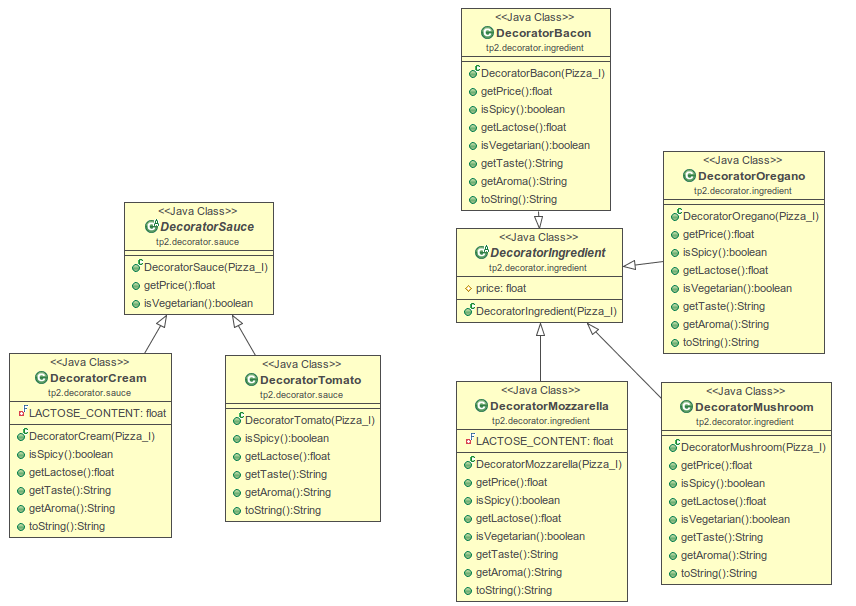
\includegraphics{decoratoringredients.png} Pour des raisons de
lisibilité, tous les decorator \texttt{DecoratorIngredient} ne sont pas
représentés

\subsection{Builder}\label{builder}

Le patron de conception \texttt{Builder} permet de créer une variété
d'objets complexes à partir d'un objet source nommé
\texttt{PizzaBuilder}.

\subsubsection{Réalisation}\label{ruxe9alisation-1}

Ce pattern est constitué en premier lieu d'une interface
\texttt{PizzaBuilder\_I} et d'une classe \texttt{PizzaBuilder} qui
représente une implémentation concrète du Builder. Nous avons également
développé un \emph{director} nommé \texttt{PizzaDirector} comme dans la
version standard du pattern qui va s'occuper de cacher la complexité du
Builder mais celui-ci n'est pas indispensable dans notre cas
d'utilisation.

Le code qui suit utilise les templates et les classes de Java. Par
exemple, pour la fonction
\texttt{setThickness(Class\textless{}?\ extends\ PizzaBase\textgreater{})},
l'utilisateur doit founir une classe qui implémente la class
\texttt{PizzaBase}. Pour pouvoir passer une classe en paramètre d'une
classe propre, il suffit de faire: \texttt{PizzaThin.class();}.

L'interface \texttt{Pizza\_I} contient les méthodes suivantes:

\begin{Shaded}
\begin{Highlighting}[]
\KeywordTok{public} \KeywordTok{interface} \NormalTok{PizzaBuilder_I \{}
    \KeywordTok{public} \DataTypeTok{void} \FunctionTok{setThickness}\NormalTok{(Class<? }\KeywordTok{extends} \NormalTok{PizzaBase> pizza);}

    \KeywordTok{public} \DataTypeTok{void} \FunctionTok{sauce}\NormalTok{(Class<? }\KeywordTok{extends} \NormalTok{DecoratorSauce> sauce);}

    \KeywordTok{public} \DataTypeTok{void} \FunctionTok{addIngredient}\NormalTok{(Class<? }\KeywordTok{extends} \NormalTok{DecoratorIngredient> ingredient);}

    \KeywordTok{public} \DataTypeTok{void} \FunctionTok{setSize}\NormalTok{(}\DataTypeTok{int} \NormalTok{radius);}

    \KeywordTok{public} \NormalTok{Pizza_I }\FunctionTok{getPizza}\NormalTok{();}
\NormalTok{\}}
\end{Highlighting}
\end{Shaded}

Finalement, voici l'implémentation de la class principale PizzaBuilder,

\begin{Shaded}
\begin{Highlighting}[]
\KeywordTok{public} \KeywordTok{class} \NormalTok{PizzaBuilder }\KeywordTok{implements} \NormalTok{PizzaBuilder_I \{}

    \KeywordTok{public} \FunctionTok{PizzaBuilder}\NormalTok{() \{}
        \KeywordTok{this}\NormalTok{.}\FunctionTok{listIngredient} \NormalTok{= }\KeywordTok{new} \NormalTok{ArrayList<Class<? }\KeywordTok{extends} \NormalTok{DecoratorIngredient>>();}
    \NormalTok{\}}

    \FunctionTok{@Override}
    \KeywordTok{public} \DataTypeTok{void} \FunctionTok{setThickness}\NormalTok{(Class<? }\KeywordTok{extends} \NormalTok{PizzaBase> pizza) \{}
        \KeywordTok{this}\NormalTok{.}\FunctionTok{pizza} \NormalTok{= pizza;}
    \NormalTok{\}}

    \FunctionTok{@Override}
    \KeywordTok{public} \DataTypeTok{void} \FunctionTok{sauce}\NormalTok{(Class<? }\KeywordTok{extends} \NormalTok{DecoratorSauce> sauce) \{}
        \KeywordTok{this}\NormalTok{.}\FunctionTok{sauce} \NormalTok{= sauce;}
    \NormalTok{\}}

    \FunctionTok{@Override}
    \KeywordTok{public} \DataTypeTok{void} \FunctionTok{addIngredient}\NormalTok{(Class<? }\KeywordTok{extends} \NormalTok{DecoratorIngredient> ingredient) \{}
        \KeywordTok{if} \NormalTok{(!listIngredient.}\FunctionTok{contains}\NormalTok{(ingredient)) \{}
            \KeywordTok{this}\NormalTok{.}\FunctionTok{listIngredient}\NormalTok{.}\FunctionTok{add}\NormalTok{(ingredient);}
        \NormalTok{\}}
    \NormalTok{\}}

    \FunctionTok{@Override}
    \KeywordTok{public} \DataTypeTok{void} \FunctionTok{setSize}\NormalTok{(}\DataTypeTok{int} \NormalTok{radius) \{}
        \KeywordTok{this}\NormalTok{.}\FunctionTok{radius} \NormalTok{= radius;}
    \NormalTok{\}}

    \FunctionTok{@Override}
    \KeywordTok{public} \NormalTok{Pizza_I }\FunctionTok{getPizza}\NormalTok{() \{}
        \CommentTok{// Build}
        \NormalTok{Pizza_I newPizza = }\KeywordTok{null}\NormalTok{;}
        \KeywordTok{try} \NormalTok{\{}
            \CommentTok{// Création de la pizza}
            \NormalTok{newPizza = (Pizza_I) pizza.}\FunctionTok{getConstructor}\NormalTok{(}\DataTypeTok{int}\NormalTok{.}\FunctionTok{class}\NormalTok{).}\FunctionTok{newInstance}\NormalTok{(}\KeywordTok{this}\NormalTok{.}\FunctionTok{radius}\NormalTok{);}

            \CommentTok{// Ajout de la sauce}
            \NormalTok{newPizza = (Pizza_I) sauce.}\FunctionTok{getConstructor}\NormalTok{(Pizza_I.}\FunctionTok{class}\NormalTok{).}\FunctionTok{newInstance}\NormalTok{(newPizza);}

            \CommentTok{// Ajout des ingrédients}
            \KeywordTok{for} \NormalTok{(Class<? }\KeywordTok{extends} \NormalTok{DecoratorIngredient> ingredient : listIngredient) \{}
                \NormalTok{newPizza = (Pizza_I) ingredient.}\FunctionTok{getConstructor}\NormalTok{(Pizza_I.}\FunctionTok{class}\NormalTok{).}\FunctionTok{newInstance}\NormalTok{(newPizza);}
            \NormalTok{\}}

        \NormalTok{\} }\KeywordTok{catch} \NormalTok{(InstantiationException | IllegalAccessException | IllegalArgumentException | InvocationTargetException}
                \NormalTok{| NoSuchMethodException | SecurityException e1) \{}
            \CommentTok{// TODO Auto-generated catch block}
            \NormalTok{e1.}\FunctionTok{printStackTrace}\NormalTok{();}
        \NormalTok{\}}
        \KeywordTok{return} \NormalTok{newPizza;}
    \NormalTok{\}}

    \CommentTok{// Input}
    \DataTypeTok{int} \NormalTok{radius;}
    \NormalTok{Class<? }\KeywordTok{extends} \NormalTok{PizzaBase> pizza;}
    \NormalTok{Class<? }\KeywordTok{extends} \NormalTok{DecoratorSauce> sauce;}
    \NormalTok{List<Class<? }\KeywordTok{extends} \NormalTok{DecoratorIngredient>> listIngredient;}
\NormalTok{\}}
\end{Highlighting}
\end{Shaded}

Notre code nous permet de créer des Builder préconfigurés pour certaines
sortes de Pizza, par exemple:

\begin{Shaded}
\begin{Highlighting}[]
\KeywordTok{public} \KeywordTok{class} \NormalTok{PizzaBuilderDiavola }\KeywordTok{extends} \NormalTok{PizzaBuilder \{}

    \KeywordTok{public} \FunctionTok{PizzaBuilderDiavola}\NormalTok{() \{}
        \KeywordTok{super}\NormalTok{();}
        \KeywordTok{this}\NormalTok{.}\FunctionTok{setSize}\NormalTok{(}\DecValTok{18}\NormalTok{);}
        \KeywordTok{this}\NormalTok{.}\FunctionTok{setThickness}\NormalTok{(PizzaThick.}\FunctionTok{class}\NormalTok{);}
        \KeywordTok{this}\NormalTok{.}\FunctionTok{sauce}\NormalTok{(DecoratorTomato.}\FunctionTok{class}\NormalTok{);}
        \KeywordTok{this}\NormalTok{.}\FunctionTok{addIngredient}\NormalTok{(DecoratorMozzarella.}\FunctionTok{class}\NormalTok{);}
        \KeywordTok{this}\NormalTok{.}\FunctionTok{addIngredient}\NormalTok{(DecoratorPepperoni.}\FunctionTok{class}\NormalTok{);}
        \KeywordTok{this}\NormalTok{.}\FunctionTok{addIngredient}\NormalTok{(DecoratorPepper.}\FunctionTok{class}\NormalTok{);}
    \NormalTok{\}}
\NormalTok{\}}
\end{Highlighting}
\end{Shaded}

Toutes les fonctions du builder sont disponibles et il est ainsi
possible de modifier le builder, lui rajouter des ingrédients, modifier
sa taille, \ldots{}

Notre implémentation nous permet de retourner une nouvelle pizza à
chaque appel de la fonction \texttt{getPizza}, certaines variantes de ce
pattern fonctionnent différemment et nécessitent de rappeler les
fonctions de constructions avant chaque nouvelle pizza car autrement ils
retournent la même pizza.

\paragraph{Diagramme de classe}\label{diagramme-de-classe-1}

\begin{figure}[htbp]
\centering
\includegraphics{Builder.jpg}
\caption{BuilderPattern}
\end{figure}

\subsubsection{Conclusion}\label{conclusion}

Notre solution remplit tous les points du cahier des charges. Ce patron
permet de simplifier la création d'objets complexes. Notre
implémentation java permet de facilement passer des classes au Builder
qui lui va s'occuper de les instancier de manière dynamique.

Cele permet de simplifier le code de l'utilisateur et de cacher toute la
complexité d'implémentation tout en offrant la possibilité de facilement
étendre le système avec l'ajout d'autres décorateurs.

\subsection{State}\label{state}

Le patron de conception \texttt{State} permet de changer le comportement
d'un objet selon l'état dans lequel il se trouve. Nous aurions pe
mdofier directement la classe \texttt{Pizza} mais cela aurait
complexifié inutilement le code.

Afin de pouvoir utiliser les contextes sur la class \texttt{Pizza}
précédemment créée, nous avons créé une classe \texttt{ContextPizza}
afin d'encapsuler notre objet pizza et modifier les différentes réponses
des fonctions de notre objet.

\subsubsection{Réalisation}\label{ruxe9alisation-2}

Pour mettre en place de ce patron, nous avons créé une interface
\texttt{State\_I} qui comporte toutes les méthodes relatives aux états
de la pizza. Ensuite, plusieurs classes d'état ont été créées sous les
noms suivants :

\begin{itemize}
\tightlist
\item
  \texttt{StateOrderer} : état commandé
\item
  \texttt{StatePrepared} : état préparé
\item
  \texttt{StateCooked} : état cuit
\item
  \texttt{StateOvercooked} : état raté
\end{itemize}

Tous ces états effectuent des tâches différentes. La classe
\texttt{PizzaContext} permet d'adapter le comportement selon l'état du
moment de la pizza.

\paragraph{Diagramme de class}\label{diagramme-de-class}

\begin{figure}[htbp]
\centering
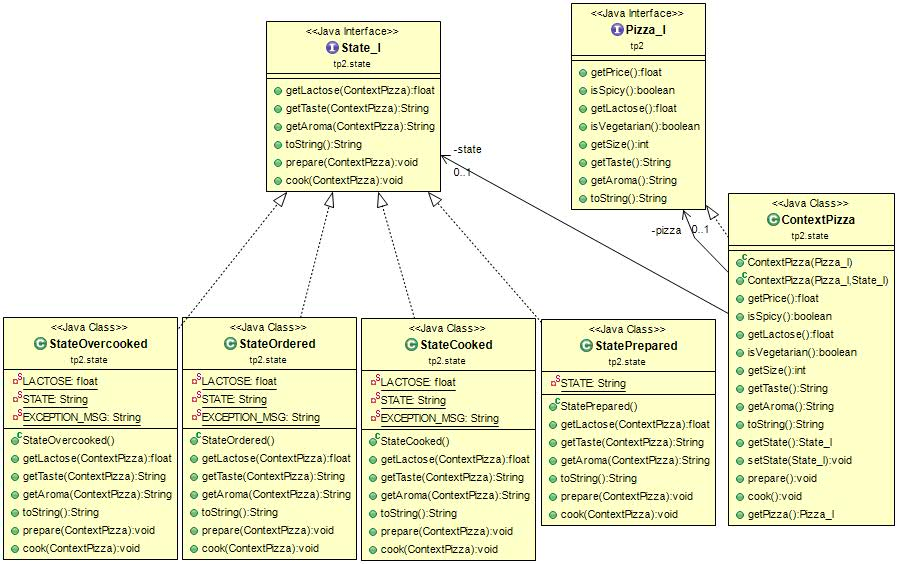
\includegraphics{StatePattern.jpg}
\caption{StatePattern}
\end{figure}

\paragraph{Exemple de code}\label{exemple-de-code-2}

\begin{Shaded}
\begin{Highlighting}[]
\CommentTok{// Interface d'état}
\KeywordTok{public} \KeywordTok{interface} \NormalTok{State_I \{}

    \KeywordTok{public} \DataTypeTok{float} \FunctionTok{getLactose}\NormalTok{(ContextPizza pizzaContext) }\KeywordTok{throws} \NormalTok{Exception;}

    \KeywordTok{public} \NormalTok{String }\FunctionTok{getTaste}\NormalTok{(ContextPizza pizzaContext) }\KeywordTok{throws} \NormalTok{Exception;}

    \KeywordTok{public} \NormalTok{String }\FunctionTok{getAroma}\NormalTok{(ContextPizza pizzaContext) }\KeywordTok{throws} \NormalTok{Exception;}

    \KeywordTok{public} \NormalTok{String }\FunctionTok{toString}\NormalTok{();}

    \KeywordTok{public} \DataTypeTok{void} \FunctionTok{prepare}\NormalTok{(ContextPizza pizzaContext) }\KeywordTok{throws} \NormalTok{Exception;}

    \KeywordTok{public} \DataTypeTok{void} \FunctionTok{cook}\NormalTok{(ContextPizza pizzaContext) }\KeywordTok{throws} \NormalTok{Exception;}
\NormalTok{\}}

\CommentTok{// Exemple d'implémentation d'un état (état commandé)}
\KeywordTok{public} \KeywordTok{class} \NormalTok{StateOrdered }\KeywordTok{implements} \NormalTok{State_I\{}

    \FunctionTok{@Override}
    \KeywordTok{public} \DataTypeTok{float} \FunctionTok{getLactose}\NormalTok{(ContextPizza pizzaContext) \{}
        \KeywordTok{return} \NormalTok{LACTOSE; }\CommentTok{// Pizza is not ready ...}
    \NormalTok{\}}

    \FunctionTok{@Override}
    \KeywordTok{public} \NormalTok{String }\FunctionTok{getTaste}\NormalTok{(ContextPizza pizzaContext) \{}
        \KeywordTok{return} \NormalTok{Tastes.}\FunctionTok{NO_TASTE}\NormalTok{.}\FunctionTok{toString}\NormalTok{();}
    \NormalTok{\}}

    \FunctionTok{@Override}
    \KeywordTok{public} \NormalTok{String }\FunctionTok{getAroma}\NormalTok{(ContextPizza pizzaContext) \{}
        \KeywordTok{return} \NormalTok{Aromas.}\FunctionTok{NO_AROMA}\NormalTok{.}\FunctionTok{toString}\NormalTok{();}
    \NormalTok{\}}

    \FunctionTok{@Override}
    \KeywordTok{public} \NormalTok{String }\FunctionTok{toString}\NormalTok{()}
    \NormalTok{\{}
        \KeywordTok{return} \NormalTok{STATE;}
    \NormalTok{\}}

    \FunctionTok{@Override}
    \KeywordTok{public} \DataTypeTok{void} \FunctionTok{prepare}\NormalTok{(ContextPizza pizzaContext) }\KeywordTok{throws} \NormalTok{Exception\{}
        \NormalTok{pizzaContext.}\FunctionTok{setState}\NormalTok{(}\KeywordTok{new} \FunctionTok{StatePrepared}\NormalTok{());}
    \NormalTok{\}}

    \FunctionTok{@Override}
    \KeywordTok{public} \DataTypeTok{void} \FunctionTok{cook}\NormalTok{(ContextPizza pizzaContext) }\KeywordTok{throws} \NormalTok{Exception\{}
        \KeywordTok{throw} \KeywordTok{new} \NormalTok{Exception(EXCEPTION_MSG);}
    \NormalTok{\}}

    \KeywordTok{private} \DataTypeTok{static} \DataTypeTok{float} \NormalTok{LACTOSE = }\FloatTok{0.}\NormalTok{0f;}
    \KeywordTok{private} \DataTypeTok{static} \NormalTok{String STATE = }\StringTok{"state : ordered"}\NormalTok{;}
    \KeywordTok{private} \DataTypeTok{static} \NormalTok{String EXCEPTION_MSG = }\StringTok{"Can not be cooked..."}\NormalTok{;}
\NormalTok{\}}

\CommentTok{// Contexte permettant d'appeler les méthodes selon l'état du moment de la pizza}
\KeywordTok{public} \KeywordTok{class} \NormalTok{ContextPizza }\KeywordTok{implements} \NormalTok{Pizza_I\{}

    \KeywordTok{public} \FunctionTok{ContextPizza}\NormalTok{(Pizza_I pizza) \{}
        \KeywordTok{this}\NormalTok{(pizza, }\KeywordTok{new} \FunctionTok{StateOrdered}\NormalTok{());}
    \NormalTok{\}}

    \KeywordTok{public} \FunctionTok{ContextPizza}\NormalTok{(Pizza_I pizza, State_I state) \{}
        \KeywordTok{this}\NormalTok{.}\FunctionTok{pizza} \NormalTok{= pizza;}
        \KeywordTok{this}\NormalTok{.}\FunctionTok{state} \NormalTok{= state;}
    \NormalTok{\}}

   \CommentTok{// ...}

    \FunctionTok{@Override}
    \KeywordTok{public} \NormalTok{String }\FunctionTok{getAroma}\NormalTok{() }\KeywordTok{throws} \NormalTok{Exception \{}
        \KeywordTok{return} \NormalTok{state.}\FunctionTok{getAroma}\NormalTok{(}\KeywordTok{this}\NormalTok{);}
    \NormalTok{\}}

    \FunctionTok{@Override}
    \KeywordTok{public} \NormalTok{String }\FunctionTok{toString}\NormalTok{() \{}
        \KeywordTok{return} \NormalTok{state.}\FunctionTok{toString}\NormalTok{() + }\StringTok{" | "} \NormalTok{+ pizza.}\FunctionTok{toString}\NormalTok{();}
    \NormalTok{\}}

    \KeywordTok{public} \NormalTok{State_I }\FunctionTok{getState}\NormalTok{()\{}
        \KeywordTok{return} \NormalTok{state;}
    \NormalTok{\}}

    \KeywordTok{public} \DataTypeTok{void} \FunctionTok{setState}\NormalTok{(State_I state) \{}
        \KeywordTok{this}\NormalTok{.}\FunctionTok{state} \NormalTok{= state;}
    \NormalTok{\}}

    \KeywordTok{public} \DataTypeTok{void} \FunctionTok{prepare}\NormalTok{() }\KeywordTok{throws} \NormalTok{Exception\{}
        \NormalTok{state.}\FunctionTok{prepare}\NormalTok{(}\KeywordTok{this}\NormalTok{);}
    \NormalTok{\}}

    \KeywordTok{public} \DataTypeTok{void} \FunctionTok{cook}\NormalTok{() }\KeywordTok{throws} \NormalTok{Exception\{}
        \NormalTok{state.}\FunctionTok{cook}\NormalTok{(}\KeywordTok{this}\NormalTok{);}
    \NormalTok{\}}

    \KeywordTok{public} \NormalTok{Pizza_I }\FunctionTok{getPizza}\NormalTok{() \{}
        \KeywordTok{return} \NormalTok{pizza;}
    \NormalTok{\}}

    \KeywordTok{private} \NormalTok{Pizza_I pizza;}
    \KeywordTok{private} \NormalTok{State_I state;}
\NormalTok{\}}
\end{Highlighting}
\end{Shaded}

\subsubsection{Conclusion}\label{conclusion-1}

L'objectif est atteint. A l'aide de ce patron, nous avons pu réaliser
une structure de programme adéquat pour le changement de comportement de
nos objets ``Pizza'' selon leur état. Ce patron s'avère très pratique
dans de telles situations. En effet, le code est beaucoup moins
``lourd'' (évite beaucoup de ``if'') et le programme se trouve mieux
structuré.

\end{document}
